\begin{figure}
  \centering
  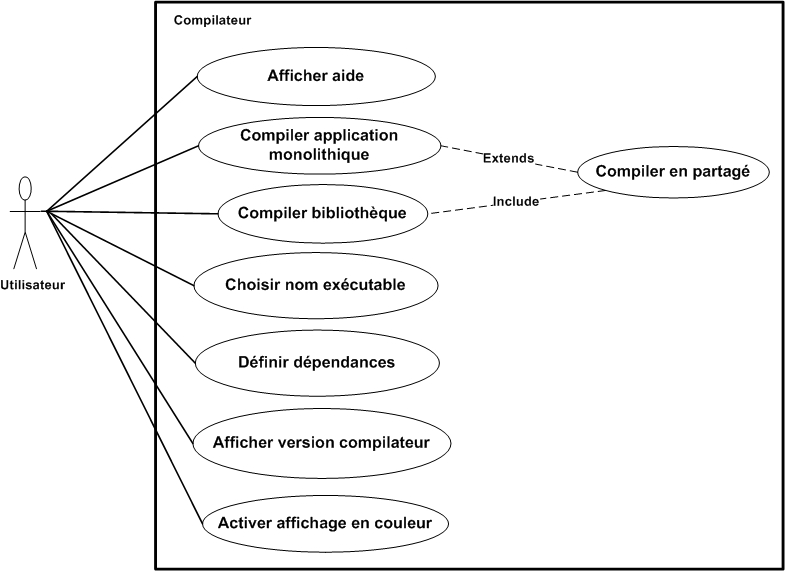
\includegraphics[scale=0.8]{../res/stb/UseCase_07.jpg}
  \caption{\textbf{Cas d'utilisations du compilateur kawa.}}
\end{figure}

%Cas d'utilisation
\subsection{Cas d'utilisation EF\_1}
\fiche
{Afficher l'aide}                    % Nom du cas d'utilisation
{Utilisateur du compilateur}                               % Acteurs concernés
{                                                % Description
  le compilateur affiche 
   la liste des options du compilateur sur la sortie standard à travers une ligne de commande.
}
{
  
}                                                % Préconditions
{Ligne de commande.}                             % Evénements déclenchants
{Action utilisateur}                       % Conditions d'arrêt
% {0.6}{../res/stb/usecase2_flot_event.png}      % Diagramme
{} % acteur(s)
{} % system
{} % flot exceptions
 % fin usecase EF_1

\subsection{Cas d'utilisation EF\_2}
\fiche
{Compiler une application en mode monolithique}                    % Nom du cas d'utilisation
{Utilisateur du compilateur}                               % Acteurs concernés
{                                                % Description
  L'utilisateur introduit un ensemble de classes
  kawa afin de les précompiler et de générer le tous dans un seul exécutable.
}
{
	Ensemble de fichiers sources 
	respectant la syntaxe du langage kawa. 
}                                                % Préconditions
{Ligne de commande.}                             % Evénements déclenchants
{Erreur (syntaxe, fichier introuvable, ..), ou 
 succès de la compilation}                       % Conditions d'arrêt
%{0.6}{../res/stb/usecase2_flot_event.png} 		 % Diagramme
{                                                % Flots d'exceptions
  
}
{} % system
{ Abondant provoqué par l'utilisateur. } % flot exceptions
% Fin de la fiche du cas d'utilisation 1.


%Cas d'utilisation 2
\subsection{Cas d'utilisation EF\_3}
\fiche
{Compiler une application en mode partagé}                    % Nom du cas d'utilisation
{Utilisateur du compilateur}                               % Acteurs concernés
{                                                % Description
  L’utilisateur introduit un ensemble de sources kawa
  ainsi des exécutables qui auraient été déjà compiler ailleurs,afin de compiler un programme kawa.
}
{
	Ensemble de fichiers source d'interfaces
	respectant la syntaxe du langage kawa. 
}                                                % Préconditions
{Ligne de commande.}                             % Evénements déclenchants
{Erreur (syntaxe, fichier introuvable, ..), ou 
 succès de la compilation}                       % Conditions d'arrêt
%{0.6}{../res/stb/usecase2_flot_event.png} 		 % Diagramme
{                                                % Flots d'exceptions
  
}{} % system
{Abondant provoqué par l'utilisateur.} % flot exceptions
% Fin de la fiche du cas d'utilisation 2.


%Cas d'utilisation
\subsection{Cas d'utilisation EF\_4}
\fiche
{Chosir un nom pour l'exécutable}                      % Nom du cas d'utilisation
{Utilisateur du compilateur}                               % Acteurs concernés
{                                                % Description
    L'utilisateur peut choisir le nom d'exécutable à produire via un ligne de commande. 
}
{
	
}                                                % Préconditions
{Ligne de commande.}                             % Evénements déclenchants
{Action utilisateur.}                       % Conditions d'arrêt
%{0.6}{../res/stb/usecase3_flot_event.png} 		 % Diagramme
{                                                % Flots d'exceptions
 
}{} % system
{} % flot exceptions
% Fin de la fiche du cas d'utilisation 3.
%Cas d'utilisation
\subsection{Cas d'utilisation EF\_5}
\fiche
{Compiler des bibliothèques}                      % Nom du cas d'utilisation
{Utilisateur du compilateur}                               % Acteurs concernés
{                                                % Description
   l'utilisateur introduit l'ensemble des sources de la  bibliothèque ce qui implique une  compilation 
   en mode partagé.Si le client ne précise pas le nom de l’exécutable, le nom est repris à partir du fichier contenant la méthode main.    
}
{
  
}                                                % Préconditions
{Ligne de commande.}                             % Evénements déclenchants
{Erreur (syntaxe, fichier introuvable, ..), ou 
 succès de la compilation.}                       % Conditions d'arrêt
%{0.6}{../res/stb/usecase3_flot_event.png}     % Diagramme
{                                                % Flots d'exceptions
 
}{} % system
{Abondant provoqué par l'utilisateur.} % flot exceptions
% Fin de la fiche du cas d'utilisation 3.
%Cas d'utilisation
\subsection{Cas d'utilisation EF\_6}
\fiche
{Afficher la version du compilateur}                      % Nom du cas d'utilisation
{Utilisateur du compilateur}                               % Acteurs concernés
{                                                % Description
   
L'utilisateur peut savoir la version du compilateur avec le quel compile ses sources et ses bibliothèques grâce à une ligne de commande.   
}
{
  
}                                                % Préconditions
{Ligne de commande.}                             % Evénements déclenchants
{Action utilisateur.}                       % Conditions d'arrêt
%{0.6}{../res/stb/usecase3_flot_event.png}     % Diagramme
{                                                % Flots d'exceptions
 
}{} % system
{} % flot exceptions
% Fin de la fiche du cas d'utilisation 3.
%Cas d'utilisation
\subsection{Cas d'utilisation EF\_7}
\fiche
{Définir des dépendances entre sources et classes}          % Nom du cas d'utilisation
{Utilisateur du compilateur}                               % Acteurs concernés
{                                                % Description
   
L'utilisateur peut définir les dépendances utiles pour la compilation entre les sources et des fichiers déjà compilés    
}
{
  
}                                                % Préconditions
{Ligne de commande.}                             % Evénements déclenchants
{Action utilisateur.}                       % Conditions d'arrêt
%{0.6}{../res/stb/usecase3_flot_event.png}     % Diagramme
{                                                % Flots d'exceptions
 
}{} % system
{} % flot exceptions
% Fin de la fiche du cas d'utilisation 3.

%Cas d'utilisation
\subsection{Cas d'utilisation EF\_8}
\fiche
{Activer l'affichage en couleur}          % Nom du cas d'utilisation
{Utilisateur du compilateur}                               % Acteurs concernés
{                                                % Description
   
L'utilisateur peut activer l'option de l'affichage en couleur, afin de décorer les messages renvoyés par le compilateur.   
}
{
  
}                                                % Préconditions
{Ligne de commande.}                             % Evénements déclenchants
{Action utilisateur.}                       % Conditions d'arrêt
%{0.6}{../res/stb/usecase3_flot_event.png}     % Diagramme
{                                                % Flots d'exceptions
 
}{} % system
{} % flot exceptions
% Fin de la fiche du cas d'utilisation 3.